\chapter{Documented Design}
\section{Introduction}
It has been decided that the new system will be a desktop application which can be used to play chess amongst two human players. It will be used by those who attend chess club to not only play games but to save, load and continue playing them. This program is to be developed in Python and for the graphical user interface Qt has been chosen, with the Pyside library serving as a python wrapper around the Qt GUI framework. 

It will consist of a visual representation of a chess board which is held in a table GUI element. This will allow players to move pieces via clicking on a piece and then on the place it wants to move the piece to. It  will contain several buttons, which all serve different functions. There will be functionality to start a new game and to save, and load, existing games. Saving a game will work by converting a python dictionary into JSON format and saving it in an existing JSON file by adding it to an array of dictionaries (games). If this file does not exist then the program will allow the user to select a location for a new JSON file to be created. This location will be saved as a setting so that the program can find this location again whenever it is relaunched.

Loading a game will open the JSON file from the location path specified by the user and scans the array of games, showing them as a table in a dialog so that the user can choose which game to open. If the location of the file does not exist, then the user will be given the option of locating a different pre-existing JSON file to open from if it exists.

As already mentioned, the JSON file will hold an array of games. A game contains the data needed to load a game: pieces and their positions, total moves, state of the game and other variables that are used to determine whether certain moves are possible, such as castling. Each game will have a unique ID which will allow users to load games that haven't been finished and to carry them on. For the program's loading and saving feature to be most useful for the school's chess club, it is best to store the JSON file in the school's shared area such that all games can be loaded and saved from any computer that has this program installed.
\section{Overall System Design}
\subsection{Input}
The first type of input is selecting a piece on the board by clicking on a cell in the $ 8\times8 $ table that contains a piece corresponding to the player's colour. At this point processing occurs and moves that are legal are added as cells that can be clicked on the table. After this, if a cell is clicked that is not a player's piece then the last clicked piece is moved to that location. If a cell is clicked that is a player's piece the process described above is repeated.

The second type of input is the player name's that must be set if the game is to be saved. Both names can be edited via 2 separate GUI TextEdit components. 

The third type of input is to do with saving and loading games. A dialog asking for the location of a JSON file (or where to save it) allows the user to select the game file for the program. When the ‘Load Button' game is pressed a dialog is shown where the user can choose a game to play from the file via a table.
\subsection{Processing}
The amount element of processing occurs when pieces are moved on the board. Once a user has used the GUI interface to declare what piece to move and to where it should be moved the main element of processing occurs. When this is done the program calculates all the possible legal moves for the opposing player's pieces. Then the GUI edits the table (which represents the chess board) such that the opponent can only select a cell in the table which represents a piece and its respective legal moves. In addition the program checks the game state and sees whether a player has won, or whether they are in check or if the game has ended in stalemate. If the game state has changed the user is informed through a dialog. 
\subsection{Storage}
All data that is required to load and save games is stored in public attributes of the Board class. When a game is saved these attributes are collated into a dictionary which is added to an array of games as a JSON file. When a game is loaded a new Board class I created where all the attributes of the loaded game are put into the class from the JSON dictionary.
\subsection{Output}
In terms of output there are three categories of output that the user will see. The first is of course the current board. The board has a visual representation of all the pieces on the correct parts of the board which is put into an 8x8 table with all cells of equal size. 

The second category is the state of the game. When the state of the game changes after a move, such as a player being in check or the game is over due to checkmate/stalemate, then the user is informed of this change by a dialog that appears. This dialog has a button to dismiss it to allow the players to continue to interact with the rest of the program, and forces users to acknowledge the change in game state.

The third category is the load dialog. The load dialog greets the user with list of games as rows on a table. The columns of the table give information about each game that is in the JSON file that the program reads from, such as the game ID, players, last played, moved made, winner etc. 
\section{Heirarchy Charts}
\subsection{Top Level View}
\begin{figure}[H]
	\centering
 	\begin{tikzpicture}
 		\node[rectangle, draw] (game) {Chess Game};
 		\node[rectangle, draw] (gameplay) [below left=of game]{Gameplay};
 		\node[rectangle, draw] (filehandling) [below right=of game]{File Handling};
 		\draw [->] (game.south) -- (gameplay.north);
 		\draw [->] (game.south) -- (filehandling.north);
 	\end{tikzpicture}
 	\caption{Top level hierarchy chart.}
\end{figure}
\subsection{Second Level View}
\begin{figure}[H]
	\centering
	\resizebox {\columnwidth} {!} {
		\begin{tikzpicture}[every node/.style={node distance= 10pt}]
		\node[rectangle, draw] (gameplay) {Gameplay};
		
		\node[rectangle, draw] (promotions) [below right=of gameplay] {Manage Promotions};
		\node[rectangle, draw] (piece-promote) [below right=of promotions] {Choose Piece to Promote};
		
		\node[rectangle, draw] (clicks) [below left=of gameplay] {Manage Table Clicks};
		\node[rectangle, draw] (select-piece) [below=of clicks] {Selecting a Piece to Move};
		\node[rectangle, draw] (move-piece) [left=of select-piece] {Moving a Piece};
		
		
		\node[rectangle, draw] (calculations) [right=of select-piece] {Game Calculations};
		\node[rectangle, draw] (game-state) [below=of calculations] {Check Game State};
		\node[rectangle, draw] (attack-move) [left=of game-state] {Attacking Moves};
		\node[rectangle, draw] (legal-move) [right=of game-state] {Legal Moves};
		
		\draw [->] (gameplay.south) -- (calculations.north);
		\draw [->] (gameplay.south) -- (clicks.north);
		\draw [->] (gameplay.south) -- (promotions.north);
		\draw [->] (clicks.south) -- (move-piece.north);
		\draw [->] (clicks.south) -- (select-piece.north);
		\draw [->] (calculations.south) -- (attack-move.north);
		\draw [->] (calculations.south) -- (game-state.north);
		\draw [->] (calculations.south) -- (legal-move.north);
		\draw [->] (promotions.south) -- (piece-promote.north);
		\end{tikzpicture}
	}
	\caption{Second level hierarchy chart: Gameplay.}
\end{figure}
\begin{figure}[H]
	\centering
	\resizebox {\columnwidth} {!} {
		\begin{tikzpicture}[every node/.style={node distance= 10pt}]
		\node[rectangle, draw] (filehandling) {Game File Handling};
		
		\node[rectangle, draw] (load-game) [below=of filehandling] {Load Game};
		
		
		\node[rectangle, draw] (save-game) [left=of load-game]{Save Game};
		\node[rectangle, draw] (create-json) [below=of save-game] {Create JSON};
		\node[rectangle, draw] (edit-json) [left=of create-json] {Edit JSON};
		
		
		\node[rectangle, draw] (filepath) [right=of load-game] {File Destination};
		\node[rectangle, draw] (filename) [below=of filepath] {Choose Filename};
		\node[rectangle, draw] (directory) [right=of filename] {Choose Directory};
		
		\node[rectangle, draw] (choose-game) [below right=of create-json] {Choose Game};
		\node[rectangle, draw] (sort-game) [right=of choose-game] {Sort Game};
		
		\draw [->] (filehandling.south) -- (load-game.north);
		\draw [->] (filehandling.south) -- (save-game.north);
		\draw [->] (filehandling.south) -- (filepath.north);
		
		\draw [->] (save-game.south) -- (edit-json.north);
		\draw [->] (save-game.south) -- (create-json.north);
		
		\draw [->] (load-game.south) -- (choose-game.north);
		\draw [->] (load-game.south) -- (sort-game.north);
		
		\draw [->] (filepath.south) -- (filename.north);
		\draw [->] (filepath.south) -- (directory.north);
		\end{tikzpicture}
	}
	\caption{Second level hierarchy chart: Game File Handling.}
\end{figure}
\section{Code Design}
\subsection{Class Diagrams}
\begin{figure}[H]
\centering
	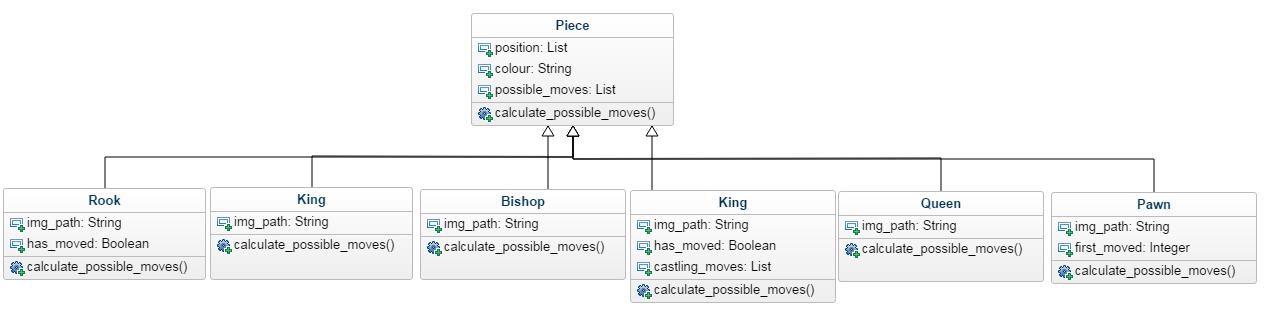
\includegraphics[width=1.0\textwidth]{images/class-diagrams/pieces}
	\caption{Class diagram for Piece and its subclasses.}
\end{figure}
\begin{figure}[H]
\centering
	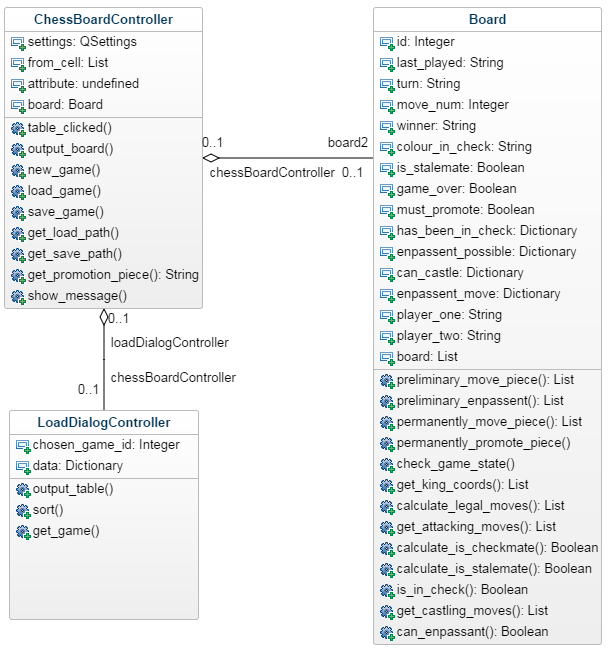
\includegraphics[width=1.0\textwidth]{images/class-diagrams/board}
	\caption{Class diagram for the controllers and model of the program.}
\end{figure}
\subsection{File and Code Structure}
As the program is in the form of a Graphical User Interface (GUI) I thought it would be appropriate to design my code around the Model-View-Controller (MVC) framework. The view of the MVC architecture is the definition of the GUI. The model is the logic of the game board and the controller is what accepts inputs and interactions with the view, which converts them to commands to the model. The results of the model processing this data is then given back to the view by the controller. The .ui file type is the file that the Qt framework generates after editing of a GUI occurs in the Qt Designer application. These are then converted to .py by a command line utility pyside-uic. I then collated these files and put them into the views.py file.
\begin{figure}[H]
	\dirtree{%
	.1 /.
	.2 src.
	.3 ui\DTcomment{Contains all the UI files }.
	.4 chessboard.ui.
	.4 loadgame.ui.
	.4 mainwindow.ui.
	.4 promotion.ui.
	.3 algorithms.py\DTcomment{Binary search and quicksort.}.
	.3 board.py\DTcomment{Contains Board class: model for the controller.}.
	.3 Chess.py\DTcomment{Starts the program when run.}.
	.3 controllers.py\DTcomment{Contains all the controllers.}.
	.3 pieces.py\DTcomment{Contains Piece class and its subclasses, used by Board class.}.
	.3 views.py\DTcomment{Contains all the views: these are generated from the .ui files.}.
	.3 resources{\_}rc.py\DTcomment{Contains image data.}.
	.3 requirements.txt\DTcomment{Contains list of all python packages that the program requires to run.}.
	}
	\caption{Code structure of the program.}
\end{figure}
\subsection{Required Software}
For this program to run via running the Chess.py file it is required that Python 3 up until 3.4 is installed on the computer that the program will be run from, anything higher is not supported. This is because the program relies on PySide being installed and it does not support versions newer than 3.4. 
\subsection{Code Documentation}
In this section the comments to all the classes and functions in the program are shown. Views.py is not commented as it is simply a compilation of .ui files that have been compiled to Python classes and Chess.py is also not commented as it is simply boilerplate code to get the GUI to run. Similarly, resources{\_}qrc.py just contains image data of the chess pieces.
\subsubsection{algorithms.py}
\begin{minted}[breaklines, breakanywhere, tabsize=4, baselinestretch=1.0, fontsize=\footnotesize]{python}
def quick_sort(array, low, high):
	"""Sorts a list recursively.

	Args:
		array (list): the list to be sorted.
		low (int): index of lowest item to be sorted.
		high (int): index of highest item to be sorted.
	"""
	def partition(array, low, high):
	"""Partitions array using a pivot value.
	
	Args:
		array (list): the list to be sorted.
		low (int): index of lowest item to be sorted.
		high (int): index of highest item to be sorted.
	
	Returns:
		The value of the pivot.
	"""

def binary_search(search_term, array):
	"""Searches for an item in an already sorted list.

	Args:
		search_term (str): term to be searched for in the list.
		array (list): list to be searched.
	
	Returns:
		True if found, False otherwise.
	"""
\end{minted}
\subsubsection{board.py}
\begin{minted}[breaklines, breakanywhere, tabsize=4, baselinestretch=1.0, fontsize=\footnotesize]{python}
class Board(object):
    """Class which manages the pieces on the board.

	This is the model for the ChessBoardController class.
	The primary function of this class is to allow the controller to determine
	the legal moves a given piece can make and to move pieces on the board, whilst
	performing checks of the game state after every move.
	
	Attributes:
		id (int): the unique identifier for a particular game.
		last_played (str): The date at which the game was last saved.
		turn (str): The colour of the current player's turn.
		move_num (int): how many moves have been made in the game.
		winner (str): The name of the winner.
		colour_in_check (str): if a player is in check, their colour is held in this variable.
		is_stalemate (bool): shows if game is in stalemate or not.
		game_over (bool): shows if game is over or not.
		must_promote (bool): true if a player must promote their pawn, false otherwise.
		enpassant_possible (dict): shows if black and white can complete an en passant move.
		enpassant_move (dict): stores the en passant move for both colours if they exist.
		player_one (str): stores the name of the first player (white).
		player_two (str): stores the name of the second player (black).
		board (list): an 8*8 2D list which maps to pieces on the board.
	"""
	
	def __init__(self, game=None):
		"""Loads a game if given one, otherwise intialises a new game.
	
		Args:
			game (dict): contains all data needed to load a game into a Board object.
		"""
		
    def new_board(self):
		"""Creates a new board."""
		
	def preliminary_move_piece(self, chess_board, old_coords, new_coords):
		""""Will move a piece temporarily. e.g. used to see if piece puts itself in check.
	
		Args:
			chess_board (list): the board to be used to move the piece.
			old_coords (list): coordinates of the piece to be moved.
			new_coords (list): coordinates of where the piece will be moved to.
		
		Returns:
			list: returns a chess board with the piece moved.
		"""
		
    def preliminary_enpassant(self, chess_board, old_coords, new_coords, removed_coords):
		"""Will perform enpassant temporarily e.g. used to see if piece puts itself in check.

		Args:
			chess_board (list): the board to be used to move the piece.
			old_coords (list): coordinates of the piece to be moved.
			new_coords (list): coordinates of where the piece will be moved to.
			removed_coords (list): coordinates of the piece to be taken.
		
		Returns:
			list: returns a chess board with the piece moved.
		"""

    def permanently_move_piece(self, chess_board, old_coords, new_coords):
		"""
		Moves a piece on the board permanently.
		It will also check for change in game state (checkmate, check, stalemate).
		
		Args:
			chess_board (list): the board to be used to move the piece.
			old_coords (list): coordinates of the piece to be moved.
			new_coords (list): coordinates of where the piece will be moved to.
		
		Returns:
			list: returns a chess board with the piece moved.
		"""
	
	def permanently_promote_piece(self, type, coords):
		"""Promotes a pawn to a piece of a certain type.
	
		Args:
			type (str): Name of the type of piece to promote to.
			coords (list): coordinates of the pawn to be promoted.
		"""

	def check_game_state(self):
		"""Completes a check of the state of the game."""
		
 	def get_king_coords(self, colour, board):
		"""Finds the coords of the king depending on its colour.
		
		Args:
			colour (str): color of the king to find.
			board (list): the board to find the kind from.
		
		Returns:
			list: coordinates of the king in the form [x,y] (0-based).
		"""
		
 	def calculate_legal_moves(self, piece):
		"""Gets all the legal moves of a piece and returns them.
	
		Args:
			piece (Piece): The piece to calculate the legal moves for.
	
		Returns:
			list: A list of all the legal moves a piece can make.
		"""
	
 	def get_attacking_moves(self, piece, board):
		"""
		Get all the attacking moves of a piece and return them.
		The difference between this function and get_legal_moves() is that
		this shows you what pieces can force a check while the other functions
		tells you whether the piece can move there.
		
		Args:
			piece (Piece): The piece to calculate the legal moves for.
			board (board): board used to determine attacking moves.
		
		Returns:
			list: A list of all attacking moves a piece can make.
		"""
	
 	def calculate_is_checkmate(self, colour, board):
		"""Finds out if a player is in checkmate.
	
		Args:
			colour (str): Colour that we are checking for if they are in checkmate.
			board (list): the board of the game being played.
		
		Returns:
			bool: True if the game is in a state of checkmate, False otherwise.
		"""
	
 	def calculate_is_stalemate(self, board):
		"""Finds out if a game is in stalemate.
	
		Args:
			board (list): the board of the game being played.
	
		Returns:
			bool: True if the game is in a state of stalemate, False otherwise.
		"""
	
 	def is_in_check(self, colour, possible_board):
		"""Checks if the king of the corresponding colour is in check.
	
		Args:
			colour (str): colour that we are checking if they are in check.
			possible_board (list): the board of the game being played.
	
		Returns:
			bool: True if the player is in check, False otherwise.
		"""
	
 	def get_castling_moves(self, king, original_board):
		"""Finds castling moves, if they exist, for a given king.
	
		Args:
			king (King): the king that we are finding castling moves for.
			original_board (list): the board of the game being played.
		"""
	
 	def can_enpassant(self, pawn, possible_board):
		"""Checks if en passant is possible, and assigns the en passant move if so.
	
		Args:
			pawn (Pawn): the pawn that we are determining if it can perform en passant.
			possible_board (list): the board of the game being played.
	
		Raises:
			IndexError: raised when index is -1 or 8 as these indices do not exist in possible_board.
		"""
\end{minted}
\subsubsection{controllers.py}
\begin{minted}[breaklines, breakanywhere, tabsize=4, baselinestretch=1.0, fontsize=\footnotesize]{python}
class MainWindowController(QtGui.QMainWindow, views.MainWindow):
	"""Controller for the main window of the application"""


class ChessBoardController(QtGui.QWidget, views.ChessBoard):
	"""Controller for the chess board.
	Attributes pertaining to the views.ChessBoard class are not listed here as there are too many
	and they merely refer to Qt GUI Objects.

	Attributes:
		board (Board): instance of the Board class which serves as the model for the controller.
		settings (QSettings): a class used to store settings (namely file path) on the host computer.
		from_cell (list): stores the coordinates of the cell that was chosen to move from.
	"""
	
	def __init__(self):
		"""Initialises necessary variables, connects click events to methods and presents a new game to the user."""
		
	def table_clicked(self):
		"""Handler for when table is clicked.
	
		When a piece has been selected to move then its legal moves are calculated.
		These moves are then made clickable and highlighted yellow.
		If a user selects any of the highlighted colours then the piece is transferred to that position
		and a check of the game state occurs where any changes are shown in a msg box.
		Promotions, if necessary, are called in this method.
		"""
		
 	def output_board(self, legal_moves=[]):
		"""Output the board onto the GUI
	
		Uses the Board.board (2D list) to help populate the QTableWidget table.
		All pieces of the moving player are made clickable on the table.
		In addition, if there are legal moves specified they are all made clickable.

		Args:
			legal_moves (list): list of the legal moves a piece can make.
		"""
	
 	def new_game(self):
		"""Creates a new game with initial board setup."""
	
 	def load_game(self):
		"""Loads a game from a JSON file. If there is no JSON file the user is prompted for one.
	
		Raises:
			IOError: raised when there is an error loading a file.
			FileNotFoundError: raised when a file is not found.
			TypeError: raised when there is an error loading a file.
			KeyError: raised when there is corruption in the JSON file.
		"""
	
 	def save_game(self):
		"""Saves a currently played game, either in an existing JSON file or a new one.
	
		Raises:
			IOError: raised when there is an error loading a file.
			FileNotFoundError: raised when a file is not found.
		"""
		
	def get_load_path(self):
		"""Gets the JSON file to load"""
		
	def get_save_path(self):
		"""Gets the desired path and filename of the file to save."""
	
 	def get_promotion_piece(self):
		"""Gets the piece that needs to be promoted"""
	
 	def show_message(self, msg):
		"""If there are errors, they are shown in a message box.
	
		Args:
			msg (str): message for the user to be shown.
		"""
		

class LoadDialogController(QtGui.QDialog, views.LoadDialog):
	"""Controller for the load dialog

	When 'Load Game' is pressed the user is shown this dialog if a JSON file is found and has been loaded.
	The user is shown a table where they can sort the games and can also choose which game to load.

	Attributes:
		chosen_game_id (int): id of the game that was chosen
		data (dict): List of games.
	"""
	
 	def __init__(self, data):
		"""Necessary variables are initialised and table is shown to the user."""
	
 	def output_table(self):
		"""List of games is shown to the user with this method."""
	
 	def sort(self):
		"""Sorts the list of games"""
	
 	def get_game(self):
		"""When game is chosen the ID is then found."""
\end{minted}
\subsubsection{pieces.py}
\begin{minted}[breaklines, breakanywhere, tabsize=4, baselinestretch=1.0, fontsize=\footnotesize]{python}
class Piece(object):
	"""Base class for all chess pieces

	Attributes:
		position (list): coordinates on the board in the form [x, y]
		colour (str): Colour of the piece, either "White" or "Black"
	"""
	
 	def __init__(self, position, colour):
		"""This constructor initialises the class variables and also calculates all possible moves for the piece."""
		
		@position.setter
		def position(self, value):
			""" This setter calculates the new possible moves once the position has changed.
		
			Args:
				value (list): coordinates on the board in the form [x, y]
			"""
	
 	def calculate_possible_moves(self):
		"""Shows us the coords it can go to assuming that there are no other pieces on the board
	
		Raises:
			NotImplementedError: Method not overridden in subclass.
		"""
		

class Rook(Piece):
	"""Class for a Rook

	Attributes:
		position (list): coordinates on the board in the form [x, y]
		colour (str): colour of the piece, either "White" or "Black"
		img_path (str): path to the image of the piece
		has_moved (bool): Denotes whether the piece has moved before.
	"""

    def __init__(self, position, colour, has_moved=False):
	"""
	This constructor initialises the class variables and also calculates all possible moves for the piece.
	In addition the image path is added.
	"""
	
 	def calculate_possible_moves(self):
		"""Calculates all the possible moves for a rook in a certain position."""
		

class Knight(Piece):
	"""Class for a Knight

	Attributes:
		position (list): coordinates on the board in the form [x, y]
		colour (str): colour of the piece, either "White" or "Black"
		img_path (str): path to the image of the piece
	"""

 	def __init__(self, position, colour):
		"""
		This constructor initialises the class variables and also calculates all possible moves for the piece.
		In addition the image path is added as an attribute self.img_path.
		"""
	
 	def calculate_possible_moves(self):
		"""Calculates all the possible moves for a knight in a certain position."""
	

class Bishop(Piece):
	"""Class for a Bishop

	Attributes:
		position (list): coordinates on the board in the form [x, y]
	colour (str): colour of the piece, either "White" or "Black"
	img_path (str): path to the image of the piece
	"""
	
	def __init__(self, position, colour):
	"""
	This constructor initialises the class variables and also calculates all possible moves for the piece.
	In addition the image path is added as an attribute self.img_path.
	"""
	
 	def calculate_possible_moves(self):
		"""Calculates all the possible moves for a bishop in a certain position."""
	

class Queen(Piece):
	"""Class for a Queen

	Attributes:
		position (list): coordinates on the board in the form [x, y]
		colour (str): colour of the piece, either "White" or "Black"
		img_path (str): path to the image of the piece
	"""

	def __init__(self, position, colour):
		"""
		This constructor initialises the class variables and also calculates all possible moves for the piece.
		In addition the image path is added as an attribute self.img_path.
		"""
	
 	def calculate_possible_moves(self):
		"""Calculates all the possible moves for a queen in a certain position."""
		

class King(Piece):
	"""Class for a King

	Attributes:
		position (list): coordinates on the board in the form [x, y].
		colour (str): colour of the piece, either "White" or "Black".
		img_path (str): path to the image of the piece.
		has_moved (bool): denotes whether piece has moved or not.
		castling_moves (list): list of all castling moves possible.
	"""

	def __init__(self, position, colour, has_moved=False, castling_moves=[]):
		"""
		This constructor initialises the class variables and also calculates all possible moves for the piece.
		In addition the image path is added as an attribute self.img_path.
		"""
	
 	def calculate_possible_moves(self):
		"""Calculates all the possible moves for a king in a certain position."""

	
class Pawn(Piece):
	"""Class for a Pawn

	Attributes:
		position (list): coordinates on the board in the form [x, y]
		colour (str): colour of the piece, either "White" or "Black"
		img_path (str): path to the image of the piece
		first_moved (int): denotes at what stage (move) in the game the the piece was first moved.
	"""

	def __init__(self, position, colour, first_moved=0):
		"""
		This constructor initialises the class variables and also calculates all possible moves for the piece.
		In addition the image path is added as an attribute self.img_path.
		"""
	
 	def calculate_possible_moves(self):
		"""Calculates all the possible moves for a pawn in a certain position."""
\end{minted}
\section{Input Validation}
\begin{table}[H]
\centering
	\resizebox{\textwidth}{!}{%
	\begin{tabular}{|p{0.25\textwidth}|p{0.2\textwidth}|p{0.3\textwidth}|p{0.25\textwidth}|}
		\hline
		\textbf{Field} & \textbf{Validation} & \textbf{Description} & \textbf{Error Message}\\ \hline
		Player names & Presence & Check for their presence & "Please fill in the player names"\\ \hline
		Path to JSON file & Valid & Checks that file exists at specified location & "File not found"\\ \hline
		Name of new JSON file & Presence/Valid & Must not contain special characters & "File not saved"\\ \hline
		Game to load & Presence & Make sure ID corresponds to existing game & Game not loaded\\ \hline
		Move to make & Move legality & Checks if a proposed move is valid & Illegal moves are not marked yellow and are not clickable on the table\\ \hline
	\end{tabular}}
	\caption{Table of information on input validation.}
\end{table}
\section{Algorithm Commentary}
In this section, algorithms used in the code base that are considered complex are fully explained.
\subsection{Binary Search}
\begin{figure}[H]
	\begin{minted}[breaklines, breakanywhere, tabsize=4, baselinestretch=1.0, fontsize=\footnotesize, linenos]{python}
		def binary_search(search_term, array):
			"""Searches for an item in an already sorted list.
	
			Args:
				search_term (str): term to be searched for in the list.
				array (list): list to be searched.
	
			Returns:
				True if found, False otherwise.
			"""
			half_array = int(len(array)/2)
			if search_term == array[half_array]:
				return True
			elif len(array) == 1:
				return False
			elif search_term > array[half_array]:
				return binary_search(search_term, array[half_array:])
			else:
				return binary_search(search_term, array[:half_array])
	\end{minted}
	\caption{Source code for the recursive binary search algorithm.}
\end{figure}

As can be noted, this algorithm is a recursive function, with recursive calls at lines 17 and 19. The function is given a sorted array and compares the middle value of the array to the search term. The base case is met when the search term is found (line 13) or if the length of the array to be searched is 1 \textbf{and} the search term is not found (line 15). If that is not the case then if the search term is larger than the middle value, then the left half of the array is passed into the same function. Otherwise the right half is passed into the same function. This carries on until the base case is met. When it is the value of \mintinline{python}/True/ or \mintinline{python}/False/ is passed up the call stack such that the first call of the function will return \mintinline{python}/True/ or \mintinline{python}/False/.
\subsection{Quicksort}
Below is the code for the recursive quicksort algorithm:
\begin{figure}[H]
	\begin{minted}[breaklines, breakanywhere, tabsize=4, baselinestretch=1.0, fontsize=\footnotesize, linenos]{python}
	def quick_sort(array, low, high):
		"""Sorts a list recursively.
	
		Args:
			array (list): the list to be sorted.
			low (int): index of lowest item to be sorted.
			high (int): index of highest item to be sorted.
		"""
		def partition(array, low, high):
			"""Partitions array using a pivot value.
	
			Args:
				array (list): the list to be sorted.
				low (int): index of lowest item to be sorted.
				high (int): index of highest item to be sorted.
	
			Returns:
				The value of the pivot.
			"""
			i = low + 1
			pivot = array[low]
			for j in range(low+1, high+1):
				if array[j] < pivot:
					array[j], array[i] = array[i], array[j]
					i += 1
				array[low], array[i-1] = array[i-1], array[low]
				return i - 1
				
		if low < high:
			pivot = partition(array, low, high)
			quick_sort(array, low, pivot-1)
			quick_sort(array, pivot+1, high)
	\end{minted}
	\caption{Source code for the recursive quicksort algorithm.}
\end{figure}
It can be noted that there is an inner function defined at line 9. Instead of defining it as another function I decided to use it as an inner function to avoid code repetition and because it has no use outside of the quicksort function. The function accepts an unsorted list, and the index of the lowest and highest element of the list to sort. The partition function is then called, where the pivot value is the first element in the list. The array is changed such that all elements smaller than the pivot are put before it, and all elements bigger are put after it. Then the quicksort function is called twice. Once for values below the pivot and for values after. Once the base case has been met for each recursive call, the list is sorted. It does not need to be returned as an array (list) in python is a mutable change and is thus changed in its scope.
\section{User Interface}
\begin{figure}[H]
	\begin{annotatedFigure}
		{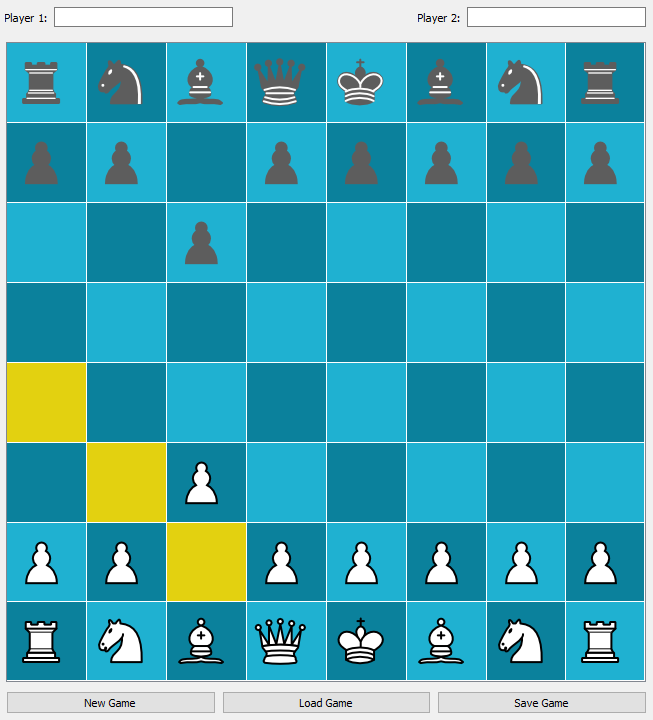
\includegraphics[width=1.0\textwidth]{images/screenshots/gui-overview}}
		\annotatedFigureBox{0.0099,0.046}{0.9924,0.95}{A}{0.0099,0.95}%tl
		\annotatedFigureBox{0.6,0.95}{0.99, 1}{B}{0.6,0.95}%bl
		\annotatedFigureBox{0.1223,0.0031}{0.2228,0.04}{C}{0.2228,0.04}%tr
		\annotatedFigureBox{0.4443,0.004}{0.5611,0.044}{D}{0.5611,0.044}%tr
		\annotatedFigureBox{0.7707,0.002}{0.8875,0.042}{E}{0.8875,0.042}%tr
	\end{annotatedFigure}
	\label{gui-overview}
	\caption{UI of the main program.}
\end{figure}
\begin{enumerate}[label=(\Alph*)]
	\item This is an $ 8\times8 $ table where input is carried out by clicking a piece then clicking again to a place where the piece is desired to be moved to. Only pieces for the player that is currently moving can be clicked. When it is clicked, all of its legal moves are made yellow, and its cells are made clickable. All the cells of illegal moves are made unclickable, which simplifies validations of moves proposed a user.
	\item This is where the name of the second player (black) is added. To the left is where the name of the first player can be added.
	\item Pressing this button starts a new game, with the board the same as in figure~\ref{initial-board}.
	\item Pressing this button results in a dialog being shown, where the user can choose which game to load. If the game file is not found then the user will be prompted to insert the file's path.
	\item Pressing this button saves the game or prompts the user for a path to save the file in.
\end{enumerate}
\begin{figure}[H]
	\centering
	\begin{annotatedFigure}
		{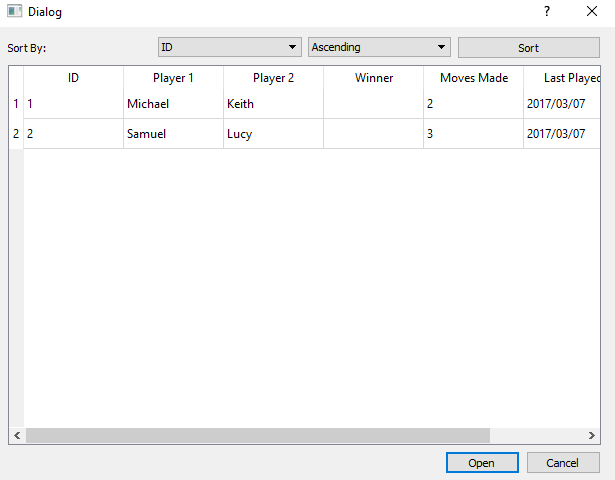
\includegraphics[width=1.0\textwidth]{images/screenshots/load-dialog}}
		\annotatedFigureBox{0.011,0.8691}{0.9805,0.9347}{A}{0.011,0.8691}%bl
		\annotatedFigureBox{0.011,0.6813}{0.9815,0.8631}{B}{0.011,0.6813}%bl
		\annotatedFigureBox{0.72,0.01}{0.9875,0.065}{C}{0.72,0.01}%tl
	\end{annotatedFigure}
	\caption{The load dialog of the program.}
\end{figure}
\begin{enumerate}[label=(\Alph*)]
	\item This section comprises of two dropdown lists, one of which determines what to sort the list of games by and the second determines whether they should be shown in ascending or descending order.
	\item This table shows the list of all of the games that are saved in the JSON file.
	\item The user can either cancel or open a game. For a game to be successfully loaded, the user must click on a game in the list and then press the 'Open' button.
\end{enumerate}
\begin{figure}[H]
\centering
	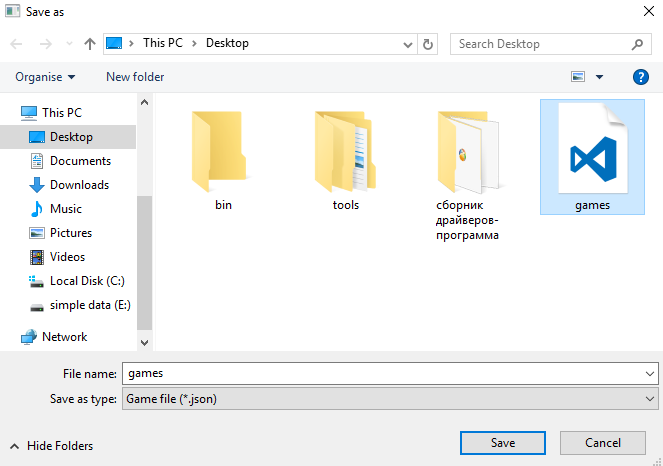
\includegraphics[width=1.0\textwidth]{images/screenshots/save-as-dialog}
	\caption{A "Save As" dialog used to save a new game file.}
\end{figure}
\begin{figure}[H]
\centering
	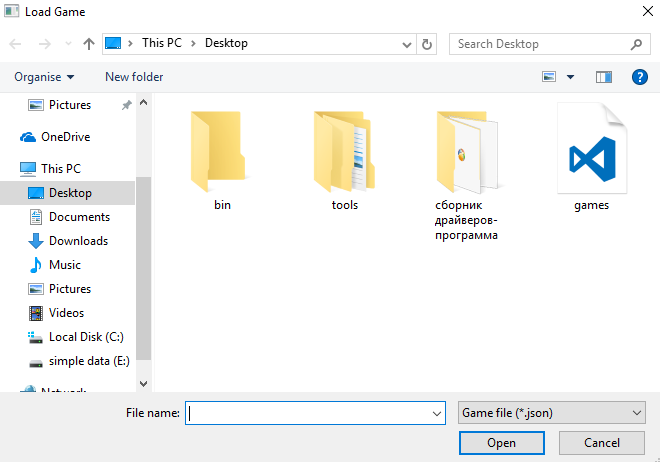
\includegraphics[width=1.0\textwidth]{images/screenshots/load-file-dialog}
	\caption{A file chooser dialog used to choose the game file to load.}
\end{figure}